% !!!IMPORTANT NOTE: Please read carefully all information including those preceded by % sign
\documentclass{aims}
\usepackage{amsmath}
  \usepackage{paralist}
  \usepackage{graphicx} %% add this and next lines if pictures should be in esp format
%  \usepackage{epsfig} %For pictures: screened artwork should be set up with an 85 or 100 line screen
% \usepackage[colorlinks=true]{hyperref}
   % Warning: when you first run your tex file, some errors might occur, please just
   % press enter key to end the compilation process,  then it will be fine if you run your tex file again.
   % Note that it is highly recommended by AIMS to use this package.
%\hypersetup{urlcolor=blue, citecolor=red}
%\usepackage{hyperref}

  \textheight=8.2 true in
   \textwidth=5.0 true in
    \topmargin 30pt
     \setcounter{page}{1}

% The next 5 line will be entered by an editorial staff.
\def\currentvolume{X}
 \def\currentissue{X}
  \def\currentyear{200X}
   \def\currentmonth{XX}
    \def\ppages{X--XX}

 % Please minimize the usage of "newtheorem", "newcommand", and use
 % equation numbers only situation when they provide essential convenience
 % Try to avoid defining your own macros

\newtheorem{theorem}{Theorem}[section]
\newtheorem{corollary}{Corollary}
\newtheorem*{main}{Main Theorem}
\newtheorem{lemma}[theorem]{Lemma}
\newtheorem{proposition}{Proposition}
\newtheorem{conjecture}{Conjecture}
\newtheorem*{problem}{Problem}
\theoremstyle{definition}
\newtheorem{definition}[theorem]{Definition}
\newtheorem{remark}{Remark}
\newtheorem*{notation}{Notation}
\newcommand{\ep}{\varepsilon}
\newcommand{\eps}[1]{{#1}_{\varepsilon}}


%% Place the running title of the paper with 40 letters or less in []
 %% and the full title of the paper in { }.
\title[Cutoffs in chaotic mixing]
      {Numerical evidence of cutoffs in chaotic mixing by the standard map}

% Place all authors' names in [ ] shown as running head;
% No more than 40 letters. Leave { } empty
% Please use `and' to connect the last two names if applicable
\author[T. Liang and M. West]{}

% It is required to enter MSC and Keywords.
\subjclass{Primary: 37M25, 65P20; Secondary: 37E30.}
 \keywords{Chaotic mixing, standard map, cutoff phenomenon.}

% 37E30   	Homeomorphisms and diffeomorphisms of planes and surfaces
% 37M25   	Computational methods for ergodic theory
% 65P20   	Numerical chaos
% 37A25   	Ergodicity, mixing, rates of mixing
% 37A50   	Relations with probability theory and stochastic processes

% Email address of each of all authors is required.
% You may list email addresses of all other authors, separately.
% \email{hartree50@gmail.com}
% \email{mwest@illinois.edu}

% Put your short thanks below. For long thanks/acknowlegements,
%please go to the last acknowlegments section.
\thanks{}

\graphicspath{{figures/}}

%%%%%%%%%%%%%%%%%%%%%%%%%%%%%%%%%%%%%%%%%%%%%%%%%%%%%%%%%%%%%%%%%%%%%%
% todo box

\usepackage{color}
\newcommand{\todo}[1]{\noindent\framebox{\begin{minipage}{0.97\columnwidth}\color{red}#1\end{minipage}}}
\newcommand{\mwtodo}[1]{\noindent\framebox{\begin{minipage}{0.97\columnwidth}\color{blue}#1\end{minipage}}}

% temporary disable todo
%\renewcommand{\todo}[1]{}

%%%%%%%%%%%%%%%%%%%%%%%%%%%%%%%%%%%%%%%%%%%%%%%%%%%%%%%%%%%%%%%%%%%%%%


\begin{document}
\maketitle

% Enter the first author's name and address:
\centerline{\scshape T. Liang}
\medskip
{\footnotesize
% please put the address of the first author
 \centerline{Department of Aeronautics and Astronautics,}
 \centerline{Stanford University,}
   \centerline{Stanford, CA 94305, USA}
} % Do not forget to end the {\footnotesize by the sign }

\medskip

\centerline{\scshape M. West}
\medskip
{\footnotesize
 % please put the address of the second  and third author
 \centerline{Department of Mechanical Science and Engineering,}
 \centerline{University of Illinois at Urbana-Champaign,}
   \centerline{Urbana, IL 61801, USA}
}

\bigskip

% The name of the associate editor will be entered by an editorial staff
% "Communicated by the associate editor name" is not needed for special issue.
% \centerline{(Communicated by the associate editor name)}


%\documentclass{article}
%\usepackage{graphicx}
%\usepackage{graphicx,psfrag}
%\usepackage{graphics}
%\usepackage{amsmath}
%\usepackage{amsthm}
%\usepackage{amsfonts}
%\title{Numerical Evidence of Cutoffs in \\Chaotic Mixing by the Standard Map}
%\author{T. Liang and M. West}
%\date{\today}
%\usepackage[margin=2.5cm]{geometry}

%\newtheorem{definition}{Definition}
%\newtheorem{conjecture}{Conjecture}


%\begin{document}

\maketitle
%%%%%%%%%%%%%%%%%%%%%%%%%%%%%%%%%%%%%%%%%%%%%%%%%%%%%%%%%%
%%%%%%%%%%%%%%%%%%%%%%%%%%%%%%%%%%%%%%%%%%%%%%%%%%%%%%%%%%
\begin{abstract}
  We numerically study the decay of the variance of a passive scalar
  function being mixed by the diffusive standard map. An efficient and
  parallelizable Markov chain model is used to approximate the
  Perron-Frobenius and Koopman operators of the chaotic map with
  diffusion. The limit of zero diffusivity is approximated by
  constructing a sequence of Markov chains with ever higher resolution
  (up to $6.4 \times 10^9$ states). In the limit of diffusivity going
  to zero we show that scalar variance exhibits a sharp decay and
  present numerical evidence to suggest that this is a cutoff in the
  sense of finite Markov chains.
\end{abstract}

%%%%%%%%%%%%%%%%%%%%%%%%%%%%%%%%%%%%%%%%%%%%%%%%%%%%%%%%%%
%%%%%%%%%%%%%%%%%%%%%%%%%%%%%%%%%%%%%%%%%%%%%%%%%%%%%%%%%%
%
% Introduction
%
\section{Introduction}
\label{sec:numcutoffintro}

It is intuitively plausible that complex dynamics causes mixing on the
state space. While this observation is crucial in many fields, such as
the study of turbulence, here we focus on two well-studied models of
this process: advection by a chaotic map and finite Markov chains. We
numerically study the chaotic standard map by constructing Markov
chain models of the dynamics and show how a connection can be made
between the chaotic mixing viewpoint and the theory of cutoff in
Markov chains.

\subsection{Mixing by chaotic maps.}
The question of how chaotic advection, often with additional
diffusion, mixes a passive scalar function has attracted much research
effort (see, e.g., \cite{Ottino2004} for a discussion). Some of the
main issues are: how to measure the thoroughness of the mixing, how
the mixing process changes qualitatively and quantitatively when the
diffusivity is close to zero, and how to enhance the overall mixing
process by designing the map which produces chaotic
advection. Unfortunately, we have only a partial understanding of most
of these topics. In spite of the fact that the detailed mechanism of
mixing is unclear, non-trivial mixing processes have been observed in
experiments \cite{Rothstein1999, Voth2002} and can be simulated by
large-scale computations \cite{topopt, Tsang2005}.

The connection between Markov chains and nonlinear dynamical systems
has been long appreciated (see, e.g., \cite{Dellnitz1999,
  Dellnitz2002, Froyland1998, Froyland1999, Froyland2001} for one
recent use). Markov chain models are simple and parallelizable and
they not only capture the multi-stage features of a chaotic mixing
process, but also provide a ready mechanism for approaching the
zero-diffusivity limit.

A widely observed phenomenon in the chaotic mixing process with small
diffusion is the two or three-stage transition
\cite{Thiffeault2003-13, Fereday2002, Antonsen1996, Mezic2005}. The
map does not mix the scalar function with a constant rate in
general. When the variance of the scalar function is measured during
the mixing process, in general we observe a relatively constant
transient initially followed by a very fast decay (together comprising
a super-exponential period), with it finally tending to a exponential
decay. We are interested in when the transitions happen between the
different phases, why they happen, and how to predict the decay rate
in the exponential region. A good review and physical interpretation
can be found in~\cite{Thiffeault2004}.

Thiffeault and Childress \cite{Thiffeault2003-13} study these
properties for a modified Arnold's cat map. Analytical formulas are
given to predict the transitions as well as the slopes. Because the
linear part of this map has an eigenvalue approximately equal to
2.618, which stretches very fast, and the chaotic part is relatively
small, the three phases are separated clearly. The same analytical
procedure cannot be applied to, for example, the standard map,
although the only difference between the standard map and the modified
Arnold's cat map is in the linear part.

As for the exponential decay part, there is still debate about whether
the decay rate goes to zero in the zero-diffusivity limit or whether
it tends to a constant independent of the diffusivity
\cite{Thiffeault2004, Tsang2005}. Theoretical analysis shows both of
these possibilities can occur for different chaotic flows
\cite{Haynes2005}.

Difficulties typically arise in studying the above problems
numerically, because the small diffusivity usually means that fine
grids are required in the solution of the advection-diffusion equation
or the simulation of the map. Some studies and numerical results
conclude that a proportional relation exists between the stationary
decay rate and the diffusivity \cite{Cerbelli2003,
  Pikovsky2003}. However, this is only true for certain diffusivity
ranges, as shown by \cite{Tsang2005}, in which the author uses a
simple and parallelizable numerical strategy which can simulate on up
to a $60\,000 \times 60\,000$ grid to show that the decay rate of a
certain chaotic map tends to a constant.

\subsection{Cutoff in Markov chains.}
Another approach to mixing can be found in the study of Markov chains,
which considers questions such as how many riffle shuffles are
required to sufficiently mix 52 cards?  This question has been
answered by Bayer and Diaconis in \cite{Diaconis1992}. It is quite
surprising that the cards are highly ordered in the first several
shuffles (6 for 52 cards) and then randomized almost abruptly. This
phenomenon has been termed \emph{cutoff}, and was discovered by
Aldous, Diaconis, and Shahshahani \cite{Diaconis1987, Diaconis1986,
  Diaconis1981}, and formalized by Aldous and Diaconis
\cite{Diaconis1996, Diaconis1987}.

The most interesting cases of cutoff are found in random walks on
finite groups with the measure of total variation distance, and most
known Markov chains that present cutoffs can be shown to belong to
this category \cite{LSaloff-Costt2004}. In general, proving the
existence of a cutoff in a certain sequence of Markov chains is a
difficult task. It usually requires some clever insight about the
system, such as the famous example of the ``rising sequence''
formulation of the riffle shuffle problem \cite{Diaconis1992}. Showing
cutoff numerically is equally difficult because it usually entails the
simulation of very large Markov chains. As a result, our knowledge
about cutoff phenomena is limited. Diaconis~\cite{Diaconis1996,
  Diaconis2005} asks, ``How widespread is the cutoff phenomenon for
families of finite ergodic Markov chains and how can one recognize
it?'' In this paper we provide a new class of Markov chains that may
exhibit cutoff phenomena (namely discretizations of chaotic maps), and
provide a numerical technique for gaining evidence that a cutoff
exists.

\subsection{Contributions and organization of this work.}
In this paper we focus on the mixing process of the standard map in
the near-zero-diffusivity limit. The two main contributions are as
follows.

First, we have produced the highest-resolution simulations of the
standard map known to date (up to an $80\,000 \times 80\,000$ grid),
allowing mixing rates to be computed with very low diffusivity. This
is achieved using a simple and parallelizable Markov chain model,
based on standard discretization methods, with a variety of diffusion
models to test the influence of discretization scheme.

Second, we explicitly connect the multiphase nature of small-diffusivity
chaotic mixing to the concept of cutoff in Markov chains, by providing
numerical evidence that cutoff seems to occur in standard map
mixing. Although there have been some historical differences in
emphasis (e.g. total variation versus $L^2$ norms used to measure
mixing), we argue that in many cases the chaotic mixing and Markov
chain cutoff problems are essentially similar. Chaotic mixing
evolution plots generally use log-scales, while Markov chain cutoffs
are typically on linear scales, making published results look
different even when the results are closely related. Another approach
to this connection is undertaken in~\cite{symdyn} using symbolic
dynamics for 1D chaotic maps.

This paper is organized as the follows: in Section~\ref{sec:evolution}
we briefly review the evolution of functions and measures by maps,
which we then discretize with Markov chain models in
Section~\ref{sec:modelreduction}. We define cutoff in
Section~\ref{sec:cutoffs-funct-evol} and then provide numerical
evidence that the standard map evolution presents a cutoff in
Section~\ref{sec:numresults}, before giving conclusions in
Section~\ref{sec:numcutoffconclusion}.

%%%%%%%%%%%%%%%%%%%%%%%%%%%%%%%%%%%%%%%%%%%%%%%%%%%%%%%%%%
%%%%%%%%%%%%%%%%%%%%%%%%%%%%%%%%%%%%%%%%%%%%%%%%%%%%%%%%%%
% body

%%%%%%%%%%%%%%%%%%%%%%%%%%%%%%%%%%%%%%%%%%%%%%%%%%%%%%%%%%
%%%%%%%%%%%%%%%%%%%%%%%%%%%%%%%%%%%%%%%%%%%%%%%%%%%%%%%%%%
\section{Function Evolution by the Standard Map}
\label{sec:evolution}
%%%%%%%%%%%%%%%%%%%%%%%%%%%%%%%%%%%%%%%%%%%%%%%%%%%%%%%%%%
%%%%%%%%%%%%%%%%%%%%%%%%%%%%%%%%%%%%%%%%%%%%%%%%%%%%%%%%%%

We work on the probability space $(X,\mathcal{A},\mu)$. We take $S: X
\to X$ to be a transformation (or map) that is non-singular and
measurable. We choose $\mu$ to be the Borel measure. In the measure
space $(X,\mathcal{A},\mu)$ we define the following operators.
%\begin{definition} {\bfseries (Markov operator)}
%Any linear operator $M:L^1 \rightarrow L^1$ satisfying
%(a) $Mf \ge 0$ for $f\ge 0, f \in L^1$; and
%(b) $||Mf|| = ||f||$ for $f\ge 0, f \in L^1$
%is called a Markov operator.
%\end{definition}

\begin{definition}[Perron-Frobenius operator]
  The \emph{Perron-Frobenius operator} or \emph{transfer operator}
  $P_S : L^1(X) \to L^1(X)$ associated with $S$ satisfies
\begin{equation}
  \int_A (P_S \omega)(x)\mu(dx) = \int_{S^{-1}(A)} \omega(x)\mu(dx)
\end{equation}
for every $\omega \in L^1(X)$ and $A \in \mathcal{A}$.
\end{definition}

The Perron-Frobenius operator is linear. Because of our choice of
measure space, the Perron-Frobenius operator can be interpreted as a
map that evolves probability density functions. Also, suppose that
$\bar{\omega}$ is an invariant measure of $S$, so that
\begin{equation}
   \bar{\omega}(S^{-1}(A)) = \bar{\omega}(A)  \text{ for all } A \in \mathcal{A}.
\end{equation}
Then we have
\begin{eqnarray}
  P_S \bar{\omega} = \bar{\omega}.
\end{eqnarray}
%Suppose $S$ is invertible and since it is measure preserving, we have
% \begin{eqnarray}
% P_Sf(x) = f(S^{-1}(x))
% \end{eqnarray}

\begin{definition}[Koopman operator]
Let $f \in L^\infty(X)$. The operator $U_S:L^{\infty}(X) \to
L^{\infty}(X)$ defined by
\begin{align}
 U_S f = f \circ S
\end{align}
is called the \emph{Koopman operator} or \emph{composition operator}
associated to $S$.
\end{definition}

The Koopman operator is linear and is adjoint to Perron-Frobenius
operator, which we write as $U_S = P_S^*$. If $S$ is invertible then
we have the following actions:
\begin{center}
\begin{tabular}{l|ll}
\label{PUtable}
& forward in time
& backward in time
\\
\hline
probability density $\omega$
& $P_S$
& $P_{S^{-1}}$
\\
scalar function $f$
& $ U_{S^{-1}} = P_{S^{-1}}^* $
& $ U_S  = P_S^*  $
\end{tabular}
\end{center}
For each probability measure $\omega \in L^1(X)$, the
\emph{multiplication operator} $T_{\omega} : L^\infty(X) \to
L^1(X)$ on scalar functions is $(T_{\omega}f)(x) = \omega(x)
f(x)$. If $\bar{\omega}$ is invariant under an invertible $S$ then we
have
\begin{align}
  \label{eqn:UPrelation}
  T_{\bar{\omega}} U_{S^{-1}} = P_S T_{\bar{\omega}}.
\end{align}
We particularly focus on the evolution of scalar functions
forward in time by the map $U_{S^{-1}}$, where the map $S$ of interest
is as follows.

\begin{definition}[Standard Map]
  The \emph{standard map} $S: [0,1]^2 \to [0,1]^2$
  is defined by $S: (x_1,x_2) \mapsto (x_1',x_2')$, with
  \begin{align}
    x_1' &= x_1+x_2' \text{ (mod 1)} \nonumber\\
    x_2' &=  x_2 +\epsilon \sin{2 \pi x_1}     \text{ (mod 1)}.
    \label{Standardmap}
  \end{align}
\end{definition}
This map is invertible and chaotic~\cite{Chirikov79, ChSh2008,
  Ott2002, LiLi1992}, where $\epsilon$ is a parameter that can be
adjusted to change the behavior of the map. Here we focus on how a
scalar function is evolved by the Koopman operator of the standard map
with the additional diffusion. A simulation of the standard map for
the initial condition $f^0(x_1,x_2)=\cos(2\pi x_2)$ is shown in
Figure~\ref{standardmapevolve}, computed using $n=500\times 500$ grid
cells and the numerical approximation $U_{S^{-1},n}^{\rm d}$ discussed
in Section~\ref{sec:modelreduction}. Because this map is volume
preserving, it has a uniform invariant measure and so $U_{S^{-1}}=P_S$
by~(\ref{eqn:UPrelation}).

\begin{figure}
  \centerline{
    \includegraphics[width=0.8\textwidth]{standardmapevolve}
  }
  \caption{\label{standardmapevolve}Evolution of the standard map with
    $\epsilon = 0.3$ and initial condition $f^0(x_1,x_2)=\cos(2\pi
    x_2)$. The simulation is with the numerical discretization
    $U_{S^{-1},n}^{\rm d}$ with $n=500 \times 500$ grid
    cells. Iterations $k = 0,1,\ldots,5$ are shown, as well as
    iterations $k = 9$ and $k = 15$.}
\end{figure}


%%%%%%%%%%%%%%%%%%%%%%%%%%%%%%%%%%%%%%%%%%%%%%%%%%%%%%%%%%
%%%%%%%%%%%%%%%%%%%%%%%%%%%%%%%%%%%%%%%%%%%%%%%%%%%%%%%%%%
\section{Markov Chain Models of Function and Measure Evolution}
\label{sec:modelreduction}
%%%%%%%%%%%%%%%%%%%%%%%%%%%%%%%%%%%%%%%%%%%%%%%%%%%%%%%%%%
%%%%%%%%%%%%%%%%%%%%%%%%%%%%%%%%%%%%%%%%%%%%%%%%%%%%%%%%%%

%%%%%%%%%%%%%%%%%%%%%%%%%%%%%%%%%%%%%%%
\subsection{A model reduction view}
%%%%%%%%%%%%%%%%%%%%%%%%%%%%%%%%%%%%%%%

In this section we explain the numerical strategy to perform the
simulation in detail. It is based on a model reduction view of
Perron-Frobenius and Koopman operators, based on \cite{ChorinHald2,
  ChorinHald1, mori1965tcm, zwanzig1980pnt, evans2008smn,
  Froyland2001, Froyland1999} (see \cite{BeLaLiWe2009} for an overview
in the finite-dimensional setting).

Given the base space $X = [0,1]^2$ of interest, we take a regular grid
with $n$ cells $a_1,a_2,\ldots,a_n$. Each cell has area $1/n$ and
dimensions $h \times h$, with $h = \sqrt{1/n}$. We are generally
interested in $n$ ranging from $500 \times 500$ up to $80\,000 \times
80\,000$. We can regard the grid as a discretization $X_n$ of the
space $X$, and we take
\begin{align}
  \label{eqn:X_n}
  X_n = \{1,2,\ldots,n\}
\end{align}
to be concrete. For any given $n$, let $g_n : X \to X_n$ be an
\emph{observation map} defined by $g_n(x) = i$ where $x \in a_i$. That
is, $g_n$ maps points to the grid cell number that they are in.

We are interested in functions and probability measures on the
discretized space $X_n$ and for clarity we write the spaces of
these as $L^\infty(X_n)$ and $L^1(X_n)$, although these are both
isomorphic to $\mathbb{R}^n$. Functions $f_n \in L^\infty(X_n)$ and
probability measures $\omega_n \in L^1(X_n)$ can thus be thought of as
vectors in $\mathbb{R}^n$ and we use the standard canonical bases
in each case, so the $i$-th coordinate of $f_n$ is $(f_n)_i = f_n(i)$.

We define the \emph{discretization} $Q_n : L^\infty(X) \to
L^\infty(X_n)$ and \emph{reconstructor} $R_n : L^\infty(X_n) \to
L^\infty(X)$ to be optimal in the sense
\begin{align}
  \label{eqn:discretization}
  Q_n f &= \operatorname*{argmin}_{f_n} \big\| f_n \circ g_n - f \big\|_{\bar{\omega}} \\
  \label{eqn:reconstructor}
  R_n f_n &= \operatorname*{argmin}_{f} \big\| f - f_n \circ g_n \big\|_{\bar{\omega}}
\end{align}
where $\bar{\omega}$ is an invariant measure of $S$ on $X$ and
$\|\cdot\|_{\bar{\omega}}$ is the $\bar{\omega}$-weighted 2-norm. In our
case these can be explicitly calculated to be
\begin{align}
  \label{eqn:discretization_particular}
  (Q_n f)_i &= \int_{a_i} f(x) \mu(dx) \\
  \label{eqn:reconstructor_particular}
  (R_n f_n)(x) &= (f_n)_{g_n(x)}
\end{align}
Note that $Q_n \circ R_n$ is the identity, but $R_n \circ Q_n$ is not.

For an evolution operator on functions, such as $U_S : L^\infty(X) \to L^\infty(X)$, we
define the \emph{optimal prediction} discretization to be a map $U_{S,n} :
L^\infty(X_n) \to L^\infty(X_n)$ satisfying
\begin{equation}
\label{objfunction1}
  U_{S,n} f_n = \operatorname*{argmin}_{f'_n}
  \big\| f'_n \circ g_n - U_S (f_n \circ g_n) \big\|_{\bar{\omega}}.
\end{equation}
That is, the optimal discretization minimizes the one-step prediction
error in the given norm. It can be shown~\cite{ChorinHald1,
  BeLaLiWe2009} that
\begin{align}
  U_{S,n} = Q_n U_S R_n.
\end{align}
The discretization $P_{S,n} : L^1(X_n) \to L^1(X_n)$ of $P_S : L^1(X)
\to L^1(X)$ is defined so that the adjoint of $P_{S,n}$ is the optimal
prediction discretization of the adjoint of $P_S$. That is,
$(P_{S,n})^* = (P_S^*)_n$. But $P_S^* = U_S$, and the adjoint for
discretized operators is simply transpose, so
\begin{align}
  P_{S,n} = U_{S,n}^T.
\end{align}

It can be shown that the optimal discretizations of $U_{S^{-1}}$ and
$P_S$ satisfy
\begin{align}
  \label{UnPnrelation}
  T_{\bar{\omega}_n} U_{S^{-1},n}
  = P_{S,n} T_{\bar{\omega}_n},
\end{align}
in analogy to~(\ref{eqn:UPrelation}), where $\bar{\omega}_n = R_n^*
\bar{\omega}$ is an invariant distribution of $P_{S,n}$
(see~\cite{BeLaLiWe2009}) and $T_{\bar{\omega}_n} :
L^\infty(X_n) \to L^1(X_n)$ is the matrix
$T_{\bar{\omega}_n} = \operatorname*{diag}(\bar{\omega}_n)$.

By construction, $P_{S,n}$ and $P_{S^{-1},n}$ are Markov matrices,
defining Markov chains on the finite state space $\mathbb{R}^n$. In
our particular case we can compute the optimal discretizations to be
\begin{align}
  (U_{S,n})_{ij} &= (P_{S,n})_{ji} = \frac{\bar{\omega}(S^{-1}(a_j)\cap a_i)}{\bar{\omega}(a_j)} \\
  (U_{S^{-1},n})_{ij} &= (P_{S^{-1},n})_{ji} = \frac{\bar{\omega}(S(a_j)\cap a_i)}{\bar{\omega}(a_j)}.
\end{align}
If the map $S$ is volume-preserving (as is the case for the Standard
Map), then, as we have remarked above, the uniform measure
$\bar{\omega}$ is invariant under $P_S$ and $P_{S^{-1}}$, and so
we also have a uniform $\bar{\omega}_n$ that is invariant under
$P_{S,n}$ and $P_{S^{-1},n}$. From~(\ref{UnPnrelation}) we then have
\begin{align}
  \label{eqn:vol_pres_Un_Pn_equal}
  U_{S^{-1},n} = P_{S,n}
\end{align}
and we see that the evolution of functions and probability measures
forward in time is identical.

For numerical efficiency, we do not use the exact expressions above
for $U_{S,n}$ or $U_{S^{-1},n}$. Instead, we recognize that if $\bar{\omega}$ is
smooth, then as $n \to \infty$ and the grid cells become very small, we have
\begin{align}
  \label{Anijapprox}
  (U_{S^{-1},n})_{ij} \approx  \frac{{\mu}(S(a_j)\cap a_i)}{\mu(a_j)}.
\end{align}
For the standard map we will use uniform invariant distributions
$\bar{\omega}$, so the approximation~(\ref{Anijapprox}) is in fact
exact for this case.

As we wish to scale to extremely high resolution, we approximate this
further. Let $C_j$ be the set of four points giving the corners of
grid cell $j$. Then we take an approximation to $U_{S^{-1},n}$ given by
\begin{align}
 \label{finegridmethod}
 (U_{S^{-1},n}^{\rm d})_{ij} = \frac{1}{4} |S(C_j) \cap a_i|,
\end{align}
where $|\cdot|$ indicates cardinality. We are thus giving weight of
$\frac{1}{4}$ to entry $(U_{S^{-1},n}^{\rm d})_{ij}$ for every corner
of cell $j$ that maps within cell $i$. It is easy to see that
$U_{S^{-1},n}^{\rm d}$ is a stochastic matrix (non-negative entries
and row-sums of 1), but it will not generally be doubly stochastic
(also having column-sums of 1), unlike the exact $U_{S^{-1},n}$.

We present numerical evidence in Section~\ref{sec:cutoff-phenomenon}
to show that the approximation of $U_{S^{-1},n}$ by $U_{S^{-1},n}^{\rm
  d}$ is unlikely to introduce any confounding influence into our
results, as we add additional diffusion which is larger than the
numerical diffusion due to any of these discretizations. We could also
adopt other discretization methods, such as the lattice method
\cite{Pierrehumbert2000}, which approximates $U_{S^{-1}}$ by a
permutation matrix, and then adds a smoothing step to make the Markov
chain irreducible. Again, however, the addition of additional
diffusion below makes the difference between the different
discretization negligible, and so using a very computationally
efficient method such as~(\ref{finegridmethod}) is a sensible choice.

In practice we do not form and store $U_{S^{-1},n}^{\rm d}$, as the
storage cost would be prohibitive. Instead we store only a state
vector $f_n$ and operate with $U_{S^{-1},n}^{\rm d}$ in a matrix-free
manner. All the numerical studies in this paper were performed on a
72-node cluster with 1~GB RAM per CPU and a gigabit ethernet
interconnect. The largest simulation ($80\,000 \times 80\,000$ grid
cells) required $51.2$~GB of memory to store a single state vector.

%%%%%%%%%%%%%%%%%%%%%%%%%%%%%%%%%%%%%%%
\subsection{Numerical and Physical Diffusion}
%%%%%%%%%%%%%%%%%%%%%%%%%%%%%%%%%%%%%%%

Using the numerical strategy from the previous section, we can evolve
a function or a probability distribution by the map with some small
error. This error manifests as numerical diffusion or smoothing with
diffusivity of the order $D \propto h^2 = 1/n$. The effect of
numerical diffusion is similar to physical diffusion on large scales,
as both cause smoothing, but their behaviors can be quite different on
small scales, and small-scale phenomena are key to mixing by chaotic
maps. To simulate physical diffusivity $D$ correctly, we need to
simulate the map with higher resolution to ensure that numerical
diffusion effects are smaller than physical diffusion. We consider two
different numerical models of physical diffusion.

First, we define the physical diffusion or spectral filter $F^{\rm
  s}_D : L^\infty(X) \to L^\infty(X)$ to be the $t=1$ evolution of the
diffusion equation with diffusivity $D$ acting on the initial
function. That is, $F^{\rm s}_D(f) = u(\cdot,1)$ where $u(x,t)$ solves
$u_{t} = D u_{xx}$ with $u(x,0) = f(x)$. Equivalently, for our case of
$X = [0,1]^2$, we can write $f(x)$ and $F^{\rm s}_D(f)(x)$ in Fourier
sine series of the form

\begin{align}
  f(x) &= \sum_{\ell_1,\ell_2=1}^\infty A_{\ell_1,\ell_2} \sin(\ell_1
  \pi x_1)
  \sin(\ell_2 \pi x_2) \\
  F^{\rm s}_D(f)(x) &= \sum_{\ell_1,\ell_2=1}^\infty w_{\ell_1,\ell_2}
  A_{\ell_1,\ell_2}
  \sin(\ell_1 \pi x_1) \sin(\ell_2 \pi x_2) \\
  w_{\ell_1,\ell_2} &= \exp\left(-4\pi^2(\ell_1^2 + \ell_2^2)
    D\right),
\end{align}
where $w_{\ell_1,\ell_2}$ are the specified weights. We write $F^{\rm
  s}_n : \mathbb{R}^n \to \mathbb{R}^n$ for the discrete analogue of
this, computed using an FFT and the same weighting coefficients with
$D = 1/n$, with a final inverse FFT.

Second, we define the finite-difference smoothing filter $F^{\rm
  f}_n$ based on~\cite{Tsang2005} by
\begin{align}
  \label{smoothingstep}
  (F^{\rm f}_n f_n)_{(p,q)} = \sum_{|r|,|s|\le 2}C_{|r|}C_{|s|}(f_n)_{(p+r,q+s)}
\end{align}
with $C_0=1/8, C_1=1/4$, and $C_2=3/16$ and $(p,q)$ the
two-dimensional index in the grid. This creates a large-scale
diffusion with diffusivity $D \propto h^2$ several times larger than
that due to numerical diffusion~\cite{Tsang2005}.

Using these different smoothing approximations, we have the following
maps:
\begin{align}
  \label{eqn:disc_approx_plain}
  U_{S^{-1},n}^{\rm d} & \text{ (no extra diffusion)} \\
  \label{eqn:disc_approx_spectral}
  U_{S^{-1},n}^{\rm d+s} &= F^{\rm s}_n U_{S^{-1},n}^{\rm d} \text{ (spectral smoothing)} \\
  \label{eqn:disc_approx_finitediff}
  U_{S^{-1},n}^{\rm d+f} &= F^{\rm f}_n U_{S^{-1},n}^{\rm d} \text{ (finite-difference smoothing)}
\end{align}
For the parameter value $\epsilon = 0.3$ in the standard map and the
initial condition $f^0(x_1,x_2)=\cos(2\pi x_2)$,
Figure~\ref{freqcompare} shows the spectral content of the iterates
$f_n^k$ versus step number $k$. Here the number of grid cells is
$n=40\,000 \times 40\,000$ and the discretized initial condition is
$f_n^0 = Q_n(f^0)$. The left plot in Figure~\ref{freqcompare} shows
iterates under the map $U_{S^{-1},n}^{\rm d}$ with no additional
diffusion (numerical diffusion only) and we observe that the chaotic
map rapidly maps low frequency components to high frequency (it also
does the converse). At this resolution $n$, the highest wavenumber
that can be meaningfully resolved is around $2 \times 10^4$, at which
point the numerical diffusion becomes dominant. The equilibrium
distribution is the result of this numerical diffusion balancing the
transport to finer scales.

\begin{figure}
  \setlength{\unitlength}{0.01\textwidth}
  \centerline{
    \begin{picture}(50,37)(0,0)
      \put(0,0){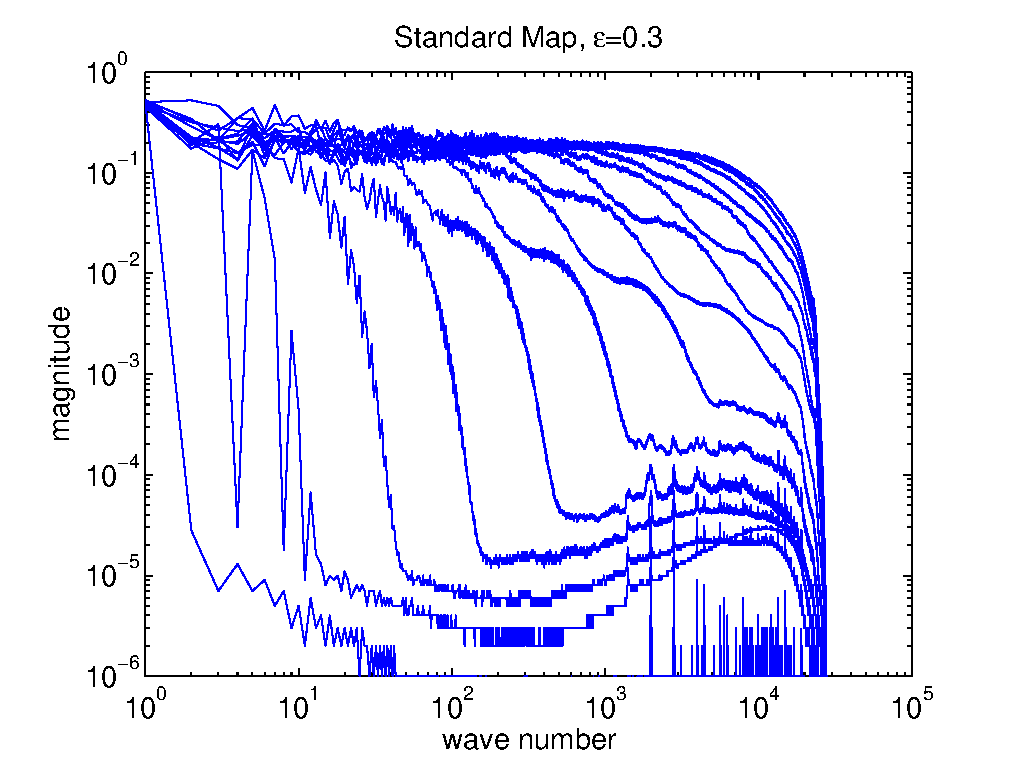
\includegraphics[width=0.5\textwidth]{standardmapfreqevolve}}
      \put(10,7){\vector(4,3){32}}
      \put(33,32){increasing $k$}
    \end{picture}
    \begin{picture}(50,37)(0,0)
      \put(0,0){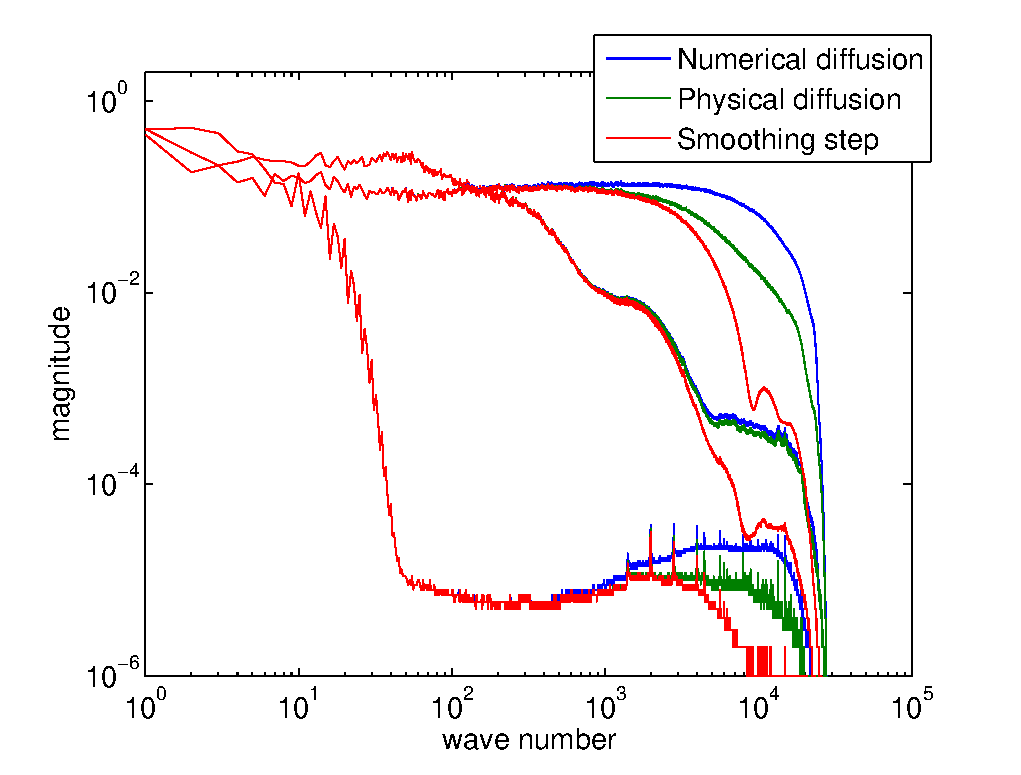
\includegraphics[width=0.5\textwidth]{standardmapfreqcompare}}
      \put(10,7){\vector(4,3){29}}
      \put(8,5){increasing $k$}
    \end{picture}
  }
  \caption{\label{freqcompare}Spatial spectral content of iterates of
    the initial condition $f^0(x_1,x_2)=\cos(2\pi x_2)$ under the
    standard map with $\epsilon = 0.3$. The number of grid cells is
    $n=40\,000 \times 40\,000$. The left plot shows the results using
    the numerical approximation $U_{S^{-1},n}^{\rm d}$ with no extra
    diffusion (numerical diffusion only) for iterates $k = 1$ through
    $20$, with the $k = 1$ line being in the lower-left, and the lines
    moving towards the upper-right as $k$ increases (as shown by the
    arrow). The right plot compares the three numerical approximations
    $U_{S^{-1},n}^{\rm d}$ (no extra diffusion), $U_{S^{-1},n}^{\rm
      d+s}$ (spectral smoothing), and $U_{S^{-1},n}^{\rm d+f}$
    (finite-difference smoothing), for iterates $k = 3$, $7$, and $20$
    (again the arrow shows the direction of increasing $k$).}
\end{figure}

To compare the difference between the operators $U_{S^{-1},n}^{\rm
  d}$, $U_{S^{-1},n}^{\rm d+f}$, and $U_{S^{-1},n}^{\rm d+s}$ with
different diffusion models, we repeated the above simulation for all
three operators. The result is plotted in the right of
Figure~\ref{freqcompare} for iterates $k = 3$, $7$, and $20$. The
three trajectories agree well at low spatial frequencies, where the
diffusion has little effect, but begin to differ around wavenumber $2
\times 10^3$. We observe that the finite difference smoothing on
$U_{S^{-1},n}^{\rm d+f}$ is greater than the spectral smoothing on
$U_{S^{-1},n}^{\rm d+s}$.

The results in Figure~\ref{freqcompare} show why it is hard to
accurately simulate the evolution of functions or measures under
chaotic maps such as the standard map. Extremely fine grids are
necessary to capture the high-frequency components generated within
just a few iterations.

In the limit $n \to \infty$ of infinite resolution, any of the maps
$U_{S^{-1},n}^{\rm d}$, $U_{S^{-1},n}^{\rm d+f}$, or
$U_{S^{-1},n}^{\rm d+s}$ are good approximations to the Standard
Map. From numerical studies in this paper, however, we used only
$U_{S^{-1},n}^{\rm d}$ and $U_{S^{-1},n}^{\rm d+f}$. This is because
they are the cheapest to compute numerically and as $U_{S^{-1},n}^{\rm
  d+s}$ has intermediate diffusivity between $U_{S^{-1},n}^{\rm d}$ and
$U_{S^{-1},n}^{\rm d+f}$, it is a reasonable supposition that because
our results hold for $U_{S^{-1},n}^{\rm d}$ and $U_{S^{-1},n}^{\rm
  d+f}$, they will hold for $U_{S^{-1},n}^{\rm d+s}$ as well. The 2D
FFT for the spectral smoothing in $U_{S^{-1},n}^{\rm d+s}$ is
expensive when $n$ is large, as on a parallel cluster the transpose
needed to switch between row and column FFTs involves much
communication.

%%%%%%%%%%%%%%%%%%%%%%%%%%%%%%%%%%%%%%%%%%%%%%%%%%%%%%%%%%%%%%%%%%%%%%
%%%%%%%%%%%%%%%%%%%%%%%%%%%%%%%%%%%%%%%%%%%%%%%%%%%%%%%%%%%%%%%%%%%%%%
\section{Variance Cutoffs in Function Evolution}
\label{sec:cutoffs-funct-evol}
%%%%%%%%%%%%%%%%%%%%%%%%%%%%%%%%%%%%%%%%%%%%%%%%%%%%%%%%%%%%%%%%%%%%%%
%%%%%%%%%%%%%%%%%%%%%%%%%%%%%%%%%%%%%%%%%%%%%%%%%%%%%%%%%%%%%%%%%%%%%%

In some Markov chains, certain probability distributions converge to
an equilibrium via a sharp transition, which becomes sharper for
larger chains. This phenomenon is referred to as \emph{cutoff} in the
finite Markov chain literature \cite{Diaconis2005, Chen2006}. Here we
modify the usual definition slightly to consider function evolution
rather than distribution evolution, and to use variance as the measure
of distance.

\begin{definition}[Variance]
  \label{def:variance}
  In a finite probability space $X_n$, the \emph{variance} of a
  function $f_n \in L^\infty(X_n)$ with respect to a probability
  measure $\omega_n \in L^1(X_n)$ is
  \begin{align}
    \label{eqn:variance}
    \operatorname{var}_{\omega_n}(f_n) = \sum_{i=1}^n (w_n)_i \left(
      (f_n)_i - \sum_{j=1}^n (\omega_n)_j (f_n)_j \right)^2.
  \end{align}
\end{definition}

We always take invariant probability measures $\bar{\omega}_n$ to
compute the variance of functions, which will be uniform measures for
the standard map. The functions we are interested in are sequences of
the form $f_n^k$, where $f_n^0 = Q_n f^0$ is the discretization of a
fixed smooth function $f^0 \in L^\infty(X)$, and $f_n^{k+1} =
U_{S^{-1},n} f_n^k$ is the time-evolution under the discretized
Koopman operator $U_{S^{-1},n}$ or one of its approximations. It is
these function sequences that we are investigating for cutoff, in the
following sense.

\begin{definition}[Cutoff]
  \label{cutoffdefinition}
  Take a family $(X_n, \omega_n,
  (f^k_n)_{k=0}^{\infty})_{n=1}^{\infty}$ of finite probability spaces
  $X_n$, probability measures $\omega_n$ on $X_n$, and sequences
  $(f_n^k)_{k=0}^{\infty}$ of functions $f_n^k$ on $X_n$. This family
  presents a \emph{variance cutoff} if there exist reals $M$ and $m$
  and a sequence $(t_n)_{n=1}^{\infty}$ of positive reals such that,
  for any $\delta \in (0,1)$, $\gamma > 1$, and sequence
  $(k_n)_{n=1}^{\infty}$,
  \begin{subequations}
    \label{eqn:defn_cutoff}
    \begin{align}
      \lim_{n \rightarrow \infty}
      \operatorname{var}_{\omega_n}(f_n^{k_n}) &= M \text{ if }
      k_n < (1-\delta)t_n \text{ for all } n \\
      \lim_{n \rightarrow \infty}
      \operatorname{var}_{\omega_n}(f_n^{k_n}) &= m \text{ if }
      k_n > (1+\delta)t_n \text{ and } k_n < \gamma t_n \text{ for all } n.
    \end{align}
  \end{subequations}
  The values $t_n$ are known as \emph{cutoff times}.
\end{definition}

This definition of cutoff is essentially the same as that for Markov
chains~\cite{Diaconis2005}, and expresses the idea that the transition
between $M$ and $m$ occurs around time $t_n$, and the time to
transition relative to $t_n$ becomes vanishingly small as $n \to
\infty$. For evolution by the standard map, we generally have a
non-zero final value $m > 0$, as the standard map has non-chaotic
regions when $\epsilon > 0$ on which fast mixing does not occur, and
on which variance decays arbitrarily slowly as $n \to \infty$. This is
also the reason for requiring $k_n/t_n$ to be bounded by a fixed
$\gamma$, as for any given $n$ it is true that
$\operatorname{var}(f_n^k) \to 0$ as $k \to \infty$.

The study of cutoff in the finite Markov chain literature began with
studying the total variation distance between an evolving probability
measure and its limiting invariant measure (see~\cite{Diaconis1996,
  Diaconis2005} for a discussion), but then also studied the
separation distance, the $L^2$ distance, and other measures of
distance. While variance~(\ref{eqn:variance}) is capturing a similar
idea to the $L^2$ distance from\cite{Diaconis2005}, the main interest
in $L^2$ cutoff for Markov chains has been for initial conditions
limiting to delta measures as $n \to \infty$~\cite{Chen2006}, whereas
we take smooth initial conditions. We study variance evolution with
smooth initial conditions because it is the most explored case in the
chaotic mixing literature (e.g.~\cite{Mezic2005,Thiffeault2003-13}).
This is also the reason we consider the evolution of functions $f_n$
rather than probability measures $\omega_n$, although for
volume-preserving maps such as the standard map we have $U_{S^{-1},n}
= P_{S,n}$ (see~(\ref{eqn:vol_pres_Un_Pn_equal})) and so this
distinction is not important. The precise statement that we believe is
true is as follows.

\begin{conjecture}
  \label{con:cutoff}
  Take the fixed smooth function $f^0 \in L^\infty(X)$ given by
  $f^0(x_1,x_2) = \cos(2\pi x_2)$ as the continuous initial
  condition. For each $n = 1,2,\ldots$, let $X_n$ be the regular grid
  with $n$ grid cells on $X = [0,1]^2$ (see~(\ref{eqn:X_n})) and
  $\omega_n$ be the uniform probability measure on $X_n$. Discretize
  the initial function with $Q_n$ (see~(\ref{eqn:discretization})) to
  give $f_n^0 = c_n Q_n f^0$, normalized by $c_n \in \mathbb{R}$ so
  that $\operatorname{var}_{\omega_n}(f_n^0) = 1$. Construct a
  sequence $(f_n^k)_{k=0}^\infty$ by evolving $f_n^{k+1} =
  U_{S^{-1},n} f_n^k$, where $U_{S^{-1},n}$ is the discretized Koopman
  operator (see~(\ref{objfunction1})) for the standard map $S$
  (see~(\ref{Standardmap})) with $\epsilon = 0.3$. Then the family
  $(X_n, \omega_n, (f^k_n)_{k=0}^{\infty})_{n=1}^{\infty}$ presents a
  variance cutoff.
\end{conjecture}

The effect of increasing the number of grid cells $n$ is to reduce the
numerical (or added) diffusivity. As we see in
Section~\ref{sec:numresults}, the cutoff behavior seems relatively
insensitive to the precise type of diffusion, and it is plausible that
cutoffs occur using any of the maps $U_{S^{-1},n}$, $U_{S^{-1},n}^{\rm
  d}$, $U_{S^{-1},n}^{\rm d+s}$, or $U_{S^{-1},n}^{\rm d+f}$. In
addition, as it is the diffusivity going to zero that causes the cutoff,
it is likely that the same behavior occurs for the continuous Koopman
operator $U_{S^{-1}}$ with smoothing, so we would expect a cutoff for
evolution by $F^{\rm s}_D U_{S^{-1}}$ as $D \to 0$, for example.

%%%%%%%%%%%%%%%%%%%%%%%%%%%%%%%%%%%%%%%%%%%%%%%%%%%%%%%%%%
%%%%%%%%%%%%%%%%%%%%%%%%%%%%%%%%%%%%%%%%%%%%%%%%%%%%%%%%%%
\section{Numerical results}
\label{sec:numresults}
%%%%%%%%%%%%%%%%%%%%%%%%%%%%%%%%%%%%%%%%%%%%%%%%%%%%%%%%%%
%%%%%%%%%%%%%%%%%%%%%%%%%%%%%%%%%%%%%%%%%%%%%%%%%%%%%%%%%%

%%%%%%%%%%%%%%%%%%%%%%%%%%%%%%%%%%%%%%%%%%%%%%%%%%%%%%%%%%
\subsection{Cutoff phenomenon}
\label{sec:cutoff-phenomenon}
%%%%%%%%%%%%%%%%%%%%%%%%%%%%%%%%%%%%%%%%%%%%%%%%%%%%%%%%%%

We now present numerical evidence for the central
Conjecture~\ref{con:cutoff} of this paper. Namely, that as the number
of grid cells $n$ of the Markov chain model of the standard map tends
to infinity, the evolution $f_n^k$ of a function tends to a trajectory
with cutoff.

To show this, we varied the number of grid cells $n$ from $2500 \times
2500$ to $80\,000 \times 80\,000$. At each resolution we took the
discretized initial condition $f_n^0 = c_n Q_n f^0$ with $f^0(x_1,x_2)
= \cos(2\pi x_2)$ and the normalization constant $c_n$ chosen so that
$\operatorname{var}(f_n^0) = 1$. We then computed iterates $f_n^k$
using both the Markov chain approximation $U_{S^{-1},n}^{\rm d}$ with
no extra diffusion, and the Markov chain approximation
$U_{S^{-1},n}^{\rm d+f}$ with finite-difference smoothing. The results
are plotted in Figure~\ref{standardmaptraj}.

\begin{figure}
    \centerline{
      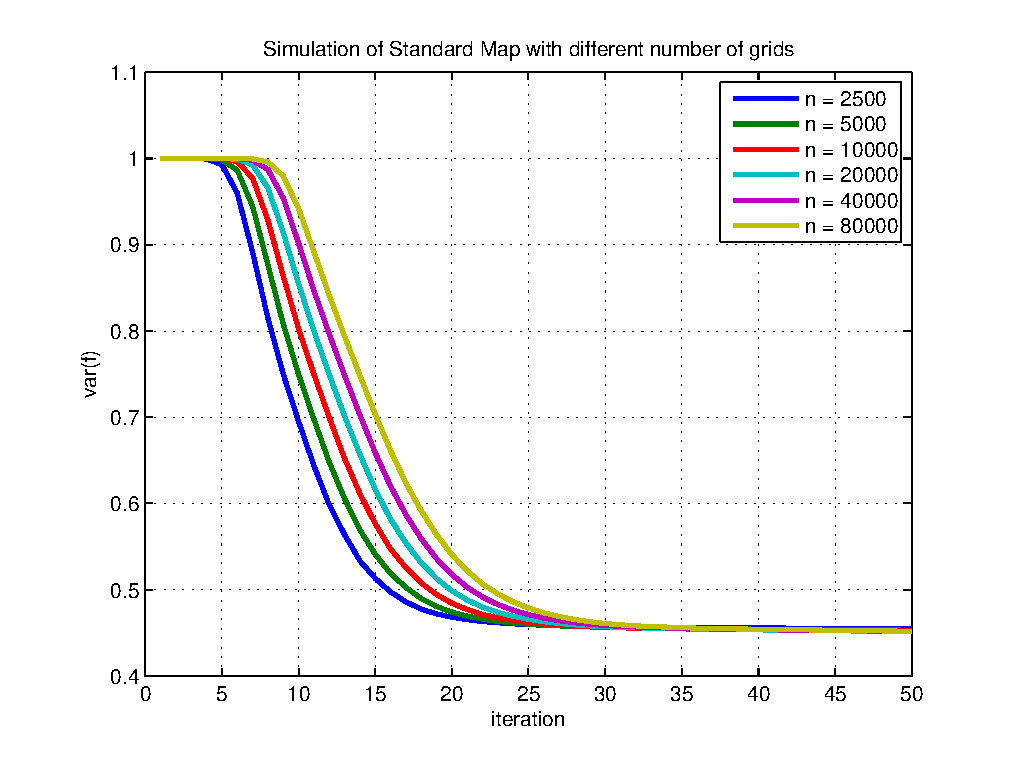
\includegraphics[width=0.5\textwidth,trim=0 0 0 22,clip=true]{standardmapcutoff}
      \includegraphics[width=0.5\textwidth,trim=0 0 0 22,clip=true]{standardmapcutoffwithsmoothing}
    }
    \caption{\label{standardmaptraj} The variance of the function
      evolved by the standard map versus iteration number, starting
      from the normalization of the initial condition
      $f^0(x_1,x_2)=\cos(2 \pi x_2)$ and with $\epsilon=0.3$. The
      standard map is modeled by the Markov chains $U_{S^{-1},n}^{\rm
        d}$ (left plot, no extra diffusion) and $U_{S^{-1},n}^{\rm
        d+f}$ (right plot, finite difference smoothing added) and the
      number of grid cells $n$ is varied from $2500 \times 2500$ to
      $80\,000 \times 80\,000$.}
\end{figure}

By construction, the variance of $f_n^k$ begins at $M = 1$. It holds
near this value for some time, before falling to a limiting value of
around $m = 0.4521$ (for $U_{S^{-1},n}^{\rm d}$) or $m = 0.4498$ (for,
$U_{S^{-1},n}^{\rm d+f}$). The variance does not drop to zero because
there are unmixed ``islands'' in the standard map. The slope of the
rapid dropping also becomes slightly milder when $n$ increases. Cutoff
occurs in the limit if the ``falling time'' becomes small relative to
the initial ``holding time''.

To make the study of this question precise in the sense of
Definition~\ref{cutoffdefinition}, we let $t_n$ equal the point where
each linearly interpolated trajectory passes through $(M+m)/2$, and we
rescaled each trajectory by scaling $t_n$ to $1$. We denote the
rescaled trajectories by $\nu_n(r)$, where $r$ represents the
normalized iteration $k / t_n$ and we linearly interpolate to make
$\nu_n(r)$ continuous for any positive $r$. The results are plotted in
Figure~\ref{standardmaptrajnorm}.

\begin{figure}
    \centerline{
      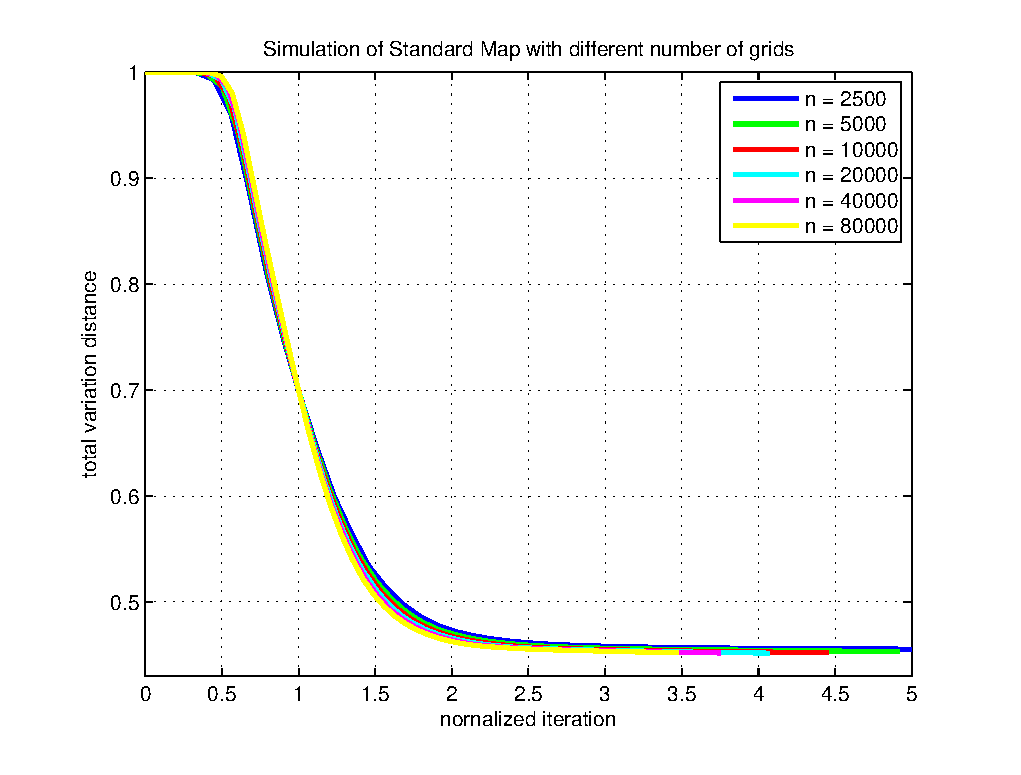
\includegraphics[width=0.5\textwidth,trim=0 0 0 22,clip=true]{standardmapcutoffn}
      \includegraphics[width=0.5\textwidth,trim=0 0 0 22,clip=true]{standardmapcutoffwithsmoothingn}
    }
    \caption{\label{standardmaptrajnorm} The trajectories from
      Figure~\ref{standardmaptraj} with iteration numbers scaled so
      the linearly interpolated trajectories at $k / t_n = 1$ are
      equal to $(M+m)/2$. The left plot is for $U_{S^{-1},n}^{\rm d}$ (no extra
      diffusion), while the right plot is for $U_{S^{-1},n}^{\rm d+f}$ (finite
      difference smoothing). The inset plots show zoomed regions near
      the corners of the trajectories.}
\end{figure}

\begin{figure}
  \centerline{
    \includegraphics[width=0.5\textwidth,trim=0 0 0 22,clip=true]{cutofftimevsD}
    \includegraphics[width=0.5\textwidth,trim=0 0 0 22,clip=true]{areavscutofftime}
  }
  \caption{\label{cutofftimeandarea} Left: the cutoff time $t_n$
    versus inverse grid cell number $1/n$, showing that the cutoff
    time is proportional to $\log(D)$ for diffusivity $D \propto
    1/n$. Right: the 1-norm distance $\Delta_n^3$ between the rescaled
    trajectories and the limiting cutoff step function, suggesting
    that the rescaled trajectories are exhibiting cutoff behavior. All
    simulations are for the standard map with parameter $\epsilon =
    0.3$, initial condition $f^0(x_1,x_2) = \cos(2\pi x_2)$, and
    number of grid cells $n$ from $2500 \times 2500$ to $80\,000
    \times 80\,000$.}
\end{figure}

Although the rescaled trajectories are very similar, we can see that
as $n$ gets larger, the rescaled trajectories becomes sharper,
suggesting that they may be tending to a cutoff. The left plot in
Figure~\ref{cutofftimeandarea} shows the cutoff times $t_n$ versus the
grid size on a semi-logarithmic plot, indicating that if there is a
cutoff, the cutoff time is inversely proportional to $\log(D)$, where
$D \propto 1/n$ is the diffusivity added by the Markov chain
approximation.

To quantify the approach of the rescaled trajectories to a sharp
cutoff, we define the limiting step function
\begin{eqnarray}
   \label{limittraj}
   \nu_{\infty}(r) = \begin{cases}
                     M &\text{if } r<1, \\
                     m &\text{otherwise}. \\
                     \end{cases} 
\end{eqnarray}
We define a 1-norm distance between the rescaled trajectories
$\nu_n(r)$ and the step function $\nu_\infty(r)$ by
\begin{eqnarray}
    \label{trajdistance}
    \Delta_n^\ell = \int_0^\ell |\nu_{\infty}(r)-\nu_{n}(r)|\,dr,
\end{eqnarray}
where $\ell$ is the length of normalized iteration under
consideration.

The right plot in Figure~\ref{cutofftimeandarea} shows $\Delta_n^\ell$
with $\ell = 3$ for both $U_{S^{-1},n}^{\rm d}$ (no extra diffusion)
and $U_{S^{-1},n}^{\rm d+f}$ (finite difference smoothing). In both
cases we see a clear and consistent trend downwards, suggesting that
$\Delta_n$ may well be converging to zero, and hence the rescaled
trajectories $\nu_n(r)$ may be limiting to the step functions
$\nu_\infty(r)$ as the number of grid cell $n$ goes to infinity, and
thus the sequences of Markov chains $U_{S^{-1},n}^{\rm d}$ and
$U_{S^{-1},n}^{\rm d+f}$ may be presenting cutoffs.

%%%%%%%%%%%%%%%%%%%%%%%%%%%%%%%%%%%%%%%%%%%%%%%%%%%%%%%%%%
\subsection{Effect of chaotic parameter $\epsilon$ and initial condition}
\label{sec:effect-chaot-param}
%%%%%%%%%%%%%%%%%%%%%%%%%%%%%%%%%%%%%%%%%%%%%%%%%%%%%%%%%%

All of the above simulations were performed with $\epsilon = 0.3$ in
the standard map equation~(\ref{Standardmap}) and the initial
condition $f^0(x_1,x_2) = \cos(2\pi x_2)$. We consider briefly here
how changing $\epsilon$ and $f^0$ might affect our conclusions.

\begin{figure}
  \centerline{
    \includegraphics[width=0.5\textwidth,trim=0 0 0 22,clip=true]{standardmapparamx}
    \includegraphics[width=0.5\textwidth,trim=0 0 0 22,clip=true]{standardmapparamy}
  }
  \caption{\label{standardmapparamxy} The evolution of function
    variance under the standard map iteration with initial condition
    $f^0(x_1,x_2) = \cos(2\pi x_1)$ (left) or $f^0(x_1,x_2) =
    \cos(2\pi x_2)$ (right), and the parameter $\epsilon$ varying
    between $0.1$ and $0.9$. All computations are performed with
    $n=40\,000 \times 40\,000$ grid cells and the discretization
    $U_{S^{-1},n}^{\rm d}$ (no extra diffusion).}
\end{figure}

We repeated the simulations with $n=40\,000 \times 40\,000$ grid cells
using the $U_{S^{-1},n}^{\rm d}$ map (no extra diffusion), taking
$\epsilon$ ranging from $0.1$ to $0.9$ and the initial condition $f^0$
being either $\cos(2\pi x_2)$ or $\cos(2\pi x_1)$. The results are
shown in Figure~\ref{standardmapparamxy}. For both initial functions
and $\epsilon \ge 0.3$, the trajectories all have similar behavior to
that observed earlier and it is likely that cutoff still occurs.

For $\epsilon=0.1$, the trajectories show no decay in the first 50
iterations for either initial condition. To explore this further, in
Figure~\ref{standardmapparamsmall} we plot the results of simulating
with $\epsilon=0$ and $0.1$ for both initial functions out to $800$
iterations.

\begin{figure}
  \centerline{
    \includegraphics[width=0.5\textwidth,trim=0 0 0 22,clip=true]{standardmapparamsmall}
  }
  \caption{\label{standardmapparamsmall} More iterations (to $k =
    800$) of the evolution of function variance under the standard map
    iteration with initial condition $f^0(x_1,x_2) = \cos(2\pi x_1)$
    or $f^0(x_1,x_2) = \cos(2\pi x_2)$, and parameter $\epsilon = 0$
    or $\epsilon = 0.1$. All computations are performed with
    $n=40\,000 \times 40\,000$ grid cells and the discretization
    $U_{S^{-1},n}^{\rm d}$ (no extra diffusion). Observe that for
    $f^0(x_1,x_2)=\cos(2\pi x_1)$, the $\epsilon=0$ trajectory crosses
    the $\epsilon=0.1$ trajectory near iteration $k = 627$.}
\end{figure}

We can see that for $f^0(x_1,x_2)= \cos(2 \pi x_2)$ and $\epsilon=0$,
the trajectory still remains almost constant $1$ for the first $800$
iterations, while in for $f^0(x_1,x_2)= \cos(2 \pi x_2)$ and
$\epsilon=0.1$ it has a small decrease but we have no evidence to say
whether a cutoff may occur.

More interesting behavior is observed for the initial condition
$f^0(x_1,x_2)= \cos(2 \pi x_1)$. In this case, the trajectory for
$\epsilon=0$ crosses over that for $\epsilon=0.1$ at around iteration
$k = 627$. This phenomenon of the $\epsilon=0$ map mixing faster than
some other trajectories with higher $\epsilon$ has also been observed
by \cite{Mezic2005}. This is because when $\epsilon=0$, there is no
unmixed region (no ``islands'') and so the decay in variance depends
only on whether the map is good at mixing the initial functions.

%%%%%%%%%%%%%%%%%%%%%%%%%%%%%%%%%%%%%%%%%%%%%%%%%%%%%%%%%%
\subsection{Zero-diffusivity limits and choice of norm}
\label{sec:zero-diff-limits}
%%%%%%%%%%%%%%%%%%%%%%%%%%%%%%%%%%%%%%%%%%%%%%%%%%%%%%%%%%

In all the above simulations, we observed how the variance of a scalar
function is evolved by the standard map with diffusion, essentially
measuring variability by the $L^2$ norm. There are many other
interesting norms that could be considered, however. In the left plot
of Figure~\ref{normcompare} we show trajectories for the following
norms: $L^1$, $L^2$, $H^{-0.5}$, $H^{-1}$, and
mix-norm~\cite{Mezic2005}. All simulations were performed using the
standard map with $\epsilon=0.3$ and initial condition $f^0(x_1,x_2)=
\cos(2\pi x_1)$ and the discretization $U_{S^{-1},n}^{\rm d}$ (no
extra diffusion) with $n=500 \times 500$ grid cells. All norms were
normalized to equal $1$ at iteration $k = 0$. Compared with the
earlier simulations, this is a very coarse grid, and so we do not
expect to see a very clear cutoff tendency. Nevertheless, these norms
do form two distinct groups of behavior: for the $L^1$ and $L^2$
norms, we observe concave trajectories for the first few iterations,
while all the other norms have trajectories that immediately decay to
around $0.5$ and then oscillate. From this we expect that we will see
cutoff in either the $L^1$ or $L^2$ norm.

\begin{figure}
  \centerline{
    \includegraphics[width=0.5\textwidth,trim=0 0 0 22,clip=true]{normcompareplot}
    \includegraphics[width=0.5\textwidth]{normcompareweighting}
  }
  \caption{\label{normcompare} Left: Different norms of $f_n^k$
    evolved by the standard map with $\epsilon=0.3$ and initial
    condition $f^0(x_1,x_2)= \cos(2\pi x_1)$. The discretization is
    $U_{S^{-1},n}^{\rm d}$ (no extra diffusion) with $n=500 \times
    500$ grid cells. The following norms of $f_n^k$ are plotted:
    $L^1$, $L^2$, $H^{-0.5}$, $H^{-1}$, and
    mix-norm~\cite{Mezic2005}. The norm trajectories form two groups:
    the $L^1$ and $L^2$ norms show the cutoff tendency seen earlier,
    while the other three norms do not.  Right: The weights of $L^2$,
    $H^{-0.5}$, $H^{-1}$, and mix-norm versus wave number in the
    frequency domain, together with the weights of the Gaussian
    diffusion operator with diffusivity $D = 0.01$ for comparison. The
    $L^2$ norm has a constant weight $1$ for all wave numbers. The
    other three norms have much smaller weights at large wave
    numbers. We see that computing the $H^{-0.5}$, $H^{-1}$, or
    mix-norm is roughly equivalent to computing the $L^2$ norm of a
    function smoothed with diffusivity $D = 0.01$.}
\end{figure}

To understand this phenomenon, let us consider the zero-diffusivity
case: the standard map is volume preserving, so without diffusion the
$L^1$ and $L^2$ norms of the scalar function will remain constant
under evolution by the Koopman operator of the standard map. The
negative Sobolev norms and the mix-norm have diagonal representations
in the frequency domain, and so can be plotted as weights for each
wavenumber, as shown in the right plot in Figure~\ref{normcompare}. We
also plot the weights of the Gaussian diffusion operator with
diffusivity $D = 0.01$ for comparison. As a function is evolved by the
Koopman operator it moves upscale in the frequency domain (as shown in
Figure~\ref{freqcompare}), and so its magnitude as measured by
$H^{-0.5}$, $H^{-1}$, or the mix-norm will decrease.

Another way to think about this is to note that the $H^{-0.5}$,
$H^{-1}$, and mix-norm of a function $f$ are very roughly equal to the
$L^2$ norm of a smoothing of $f$, where the smoothing is performed by
the diffusion operator with $D \approx 0.01$. This diffusivity is very
large and far from entering the range where we are seeing potential
cutoff behavior. That is, the norms $H^{-0.5}$, $H^{-1}$, and mix-norm
are explicitly insensitive to high-wavenumber (small-scale)
information, but it is precisely the high-wavenumber behavior of the
chaotic map that is responsible for cutoff. It is thus not surprising
that these three norms do not exhibit a cutoff.

We stress that there is no one norm that is ``better'' than another
for measuring mixing. They simply give different information about the
mixing process. The concave trajectories of $L^1$ and $L^2$ norms
indicate the ``irreversibility'' of the chaotic system with small
diffusivity: beyond the cutoff time substantial information about the
initial system state has been lost. In contrast, the fast decay of the
other norms shows the increasing complexity of the function evolved by
the chaotic map in the first few iterations, but does not indicate
when the initial state information has been lost.

%%%%%%%%%%%%%%%%%%%%%%%%%%%%%%%%%%%%%%%%%%%%%%%%%%%%%%%%%%
%%%%%%%%%%%%%%%%%%%%%%%%%%%%%%%%%%%%%%%%%%%%%%%%%%%%%%%%%%

\section{Conclusion}
\label{sec:numcutoffconclusion}

We have presented the highest-resolution numerical simulations of the
standard map known to date, and thereby provided numerical evidence of
a cutoff in the sequence of Markov chains generated by approximating
the Koopman operator of the standard map. The notion of a cutoff was taken
from the study of finite Markov chains and applied to the study of
chaotic mixing. We showed that cutoff not only characterizes the
behavior of diffusive chaotic maps in the near-zero-diffusivity limit,
but it also builds a bridge between the study of large finite Markov
chains and chaotic maps.

Many Markov chains with cutoff are known, such as random walks on
hypercubes or riffle-shuffling of cards, and it is not yet clear
whether such chains can be related to chaos: are they discretizations
or approximations of some chaotic map? We offer no good answer to this
question so far. However, in \cite{symdyn} another attempt is made: we
show that by choosing suitable initial distributions, a $1$D chaotic
map with symbolic dynamics can have the same limiting behavior as the
cutoff of a random walk on $n$-dimensional hypercube
problem~\cite{Diaconis1990}, and thus it demonstrates another link
between these chaotic mixing and cutoff.

The results in the paper have focused on variance as the measure of
mixing, but as discussed in Section~\ref{sec:zero-diff-limits}, it
seems likely that similar results will occur for $L^1$ distances, and
we do not expect cutoffs using negative Sobolov norms. This emphasizes
the well-known fact that the details of mixing behavior are highly
dependent on the definition of mixing.

We have also considered only finite dimensional Markov chains in the
present study, due to the numerical nature of our techniques. From
Section~\ref{sec:cutoff-phenomenon} we saw that the results are
insensitive to the details of the discretization and the type of
diffusion. From this, we expect that the true Koopman evolution
$U_{S^{-1}}$ with diffusion $F^{\rm s}_D$, giving the map $F^{\rm s}_D
U_{S^{-1}}$, will also present a cutoff as $D \to 0$.

%%%%%%%%%%%%%%%%%%%%%%%%%%%%%%%%%%%%%%%%%%%%%%%%%%%%%%%%%%
%%%%%%%%%%%%%%%%%%%%%%%%%%%%%%%%%%%%%%%%%%%%%%%%%%%%%%%%%%

% References
 %\bibliographystyle{plain}
 \bibliographystyle{abbrv}
\bibliography{../mixingbib}

\end{document}
